
很多开发者在学习上一节的内容时,第一反应通常是这样的:“谢谢,我现在理解了为什么我的程序很慢,但我必须处理我的数据,不只是理想的32KB,算法就是这样,包括复杂的数据访问模式,所以我无能为力。”如果我们不了解如何为需要解决的问题获得更好的内存性能,那么这一章就没有多大存在意义。本节中,我们将了解可以用来提高内存性能的技术。

\subsubsubsection{4.5.1\hspace{0.2cm}节约内存数据结构}

就内存性能而言,数据结构或数据组织的选择通常是开发者所做的重要的决策。重要的是要理解你能做什么和不能做什么:图4.5和图4.6展示了内存性能,这里不能绕过它(严格地说,这是99\%的正确;有一些奇异的内存访问技术,很少会超过这些图中所示的限制)。但可以在这些图上选择与自己程序相对应的点。首先考虑一个简单的示例:我们有1M个64位的整数,需要按顺序存储和处理。我们可以将这些值存储在数组中,数组的大小将为8MB。根据我们的测量,每个值的访问时间约为0.6纳秒,如图4.6所示。

%\hspace*{\fill} \\ %插入空行
\begin{center}
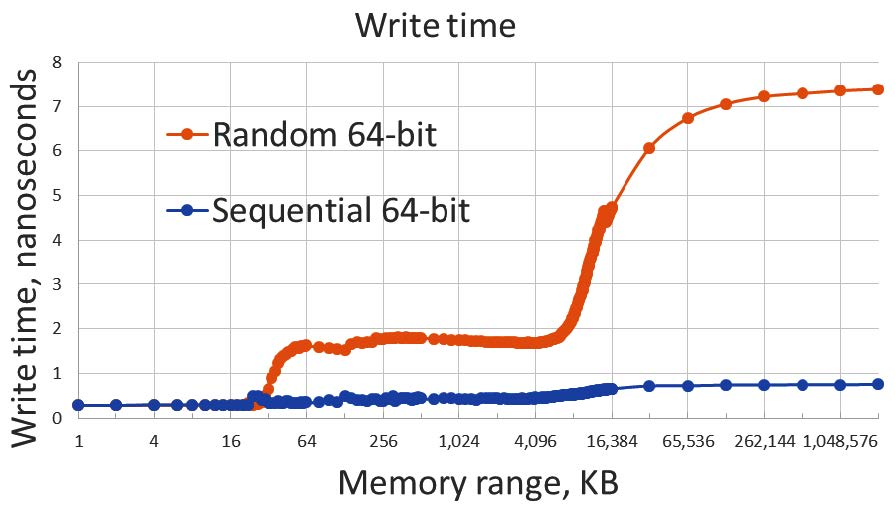
\includegraphics[width=0.9\textwidth]{content/1/chapter4/images/9.jpg}\\
图4.9 - 写入数组(A)[随机]和列表(L)[顺序]的时间
\end{center}

首先,可以使用列表来存储。\texttt{std::list}是节点的集合,每个节点都有一个值和两个指向下一个和上一个节点的指针。因此,整个列表使用24MB的内存。此外,每个节点通过对\texttt{operator new}的单独调用来分配,因此不同的节点可能位于非常不同的地址,特别是当程序同时进行其他内存分配和回收时。在遍历这个列表时,需要访问的地址没有任何模式,所以要找到这个列表的性能点,我们需要做的就是在曲线上找到对应于随机内存访问的24MB内存范围的点。这使得每个值只比访问数组中的相同数据慢了5纳秒或一个数量级。

这些,前一章已经证明。我们可以很容易地构造一个微基准来比较将数据写入相同大小的列表和数组的区别。以下是数组的基准测试:

\hspace*{\fill} \\ %插入空行
\noindent
\textbf{03\_list\_vector.C}
\begin{lstlisting}[style=styleCXX]
template <class Word>
void BM_write_vector(benchmark::State& state) {
	const size_t size = state.range(0);
	std::vector<Word> c(size);
	Word x = {};
	for (auto _ : state) {
		for (auto it = c.begin(), it0 = c.end(); it !=
		it0;) {
			REPEAT(benchmark::DoNotOptimize(*it++ = x);)
		}
		benchmark::ClobberMemory();
	}
}
BENCHMARK_TEMPLATE1(BM_write_vector, unsigned long)-
>Arg(1<<20);
\end{lstlisting}

将\texttt{std::vector}改为\texttt{std::list}来创建一个基准测试。与之前的基准测试相比,现在是容器中元素的数量已经发生了变化,因此内存大小将取决于元素类型和容器本身,如图4.6所示。对于1M个元素,结果与预期完全一致:

%\hspace*{\fill} \\ %插入空行
\begin{center}
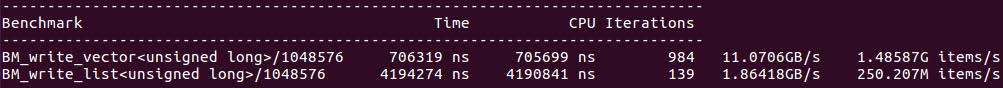
\includegraphics[width=0.9\textwidth]{content/1/chapter4/images/10.jpg}\\
图4.10 - 列表和数组的基准测试结果
\end{center}

为什么会有人选择列表而不是数组(或\texttt{std::vector})?最常见的原因是,在创建时不知道有多少数据,并且由于涉及复制,增长\texttt{std::vector}的效率非常低。有几种方法可以解决这个问题,有时可以预先计算出数据的最终大小,例如:需要对输入数据进行一次扫描,以确定为结果分配多少空间。如果有效地组织了输入,那么可能值得对输入进行两次传递:第一次是计数,第二次是进行处理。

如果不能提前知道最终的数据大小,可能需要一种更智能的数据结构,将\texttt{vector}的内存与\texttt{list}的调整大小效率结合起来。这可以通过使用块分配数组来实现:

%\hspace*{\fill} \\ %插入空行
\begin{center}
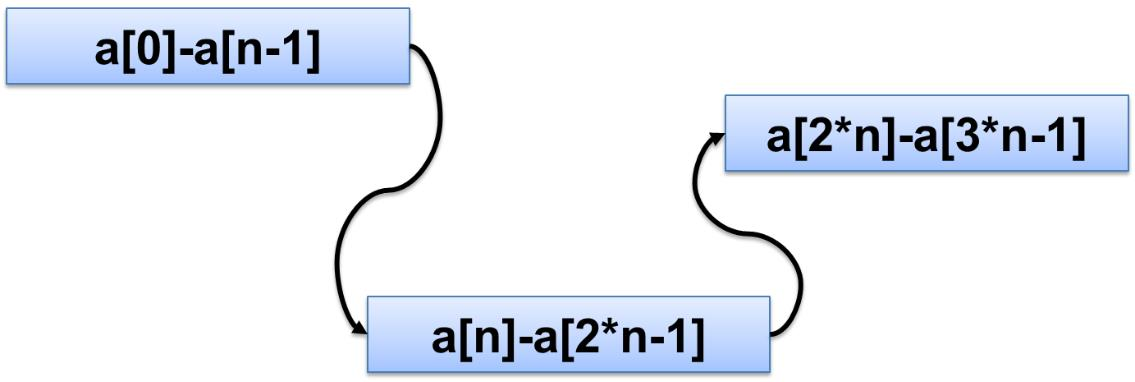
\includegraphics[width=0.8\textwidth]{content/1/chapter4/images/11.jpg}\\
图4.11 - 块分配的数组(deque)可以在适当的位置进行增长
\end{center}

这种数据结构以固定数量的块分配内存,通常小到足以装入L1缓存(通常在2KB到16KB之间)。每个块都用作数组,因此每个块中,将顺序访问元素,而块本身在在一个列表中。我们需要扩展这个数据结构,只分配一个块,并将其添加到列表中。访问每个块的第一个元素很可能会导致缓存丢失,但是当预取检测到顺序访问的模式时,块中的其他元素可以高效地访问到。按每个块中的元素数量平摊,随机访问的代价可以变得非常小,结果数据结构的性能几乎与数组或向量相同。在STL中,我们有这样一个数据结构:\texttt{std::deque}(不幸的是,大多数STL版本的实现不是特别高效,顺序访问\texttt{deque}通常比访问相同大小的\texttt{vector}慢一些)。

另一个选择列表而不是数组、单块或块分配的原因是,列表允许在任何点进行快速插入,而不仅仅是在末尾。如果需要,必须使用列表或另一个节点分配的容器。这种情况下,最好的解决方案通常不是尝试选择一个适合所有需求的数据结构,而是将数据从一个数据结构迁移到另一个数据结构,例如:如果想使用列表来存储数据元素,每次存储一个,同时保持排序顺序,那么问题来了,我们是否需要在所有元素插入后,对该顺序进行排序?还是,需要在构建过程的中间进行几次排序,而不是一直进行排序?

如果算法中发生了数据访问模式的改变,那么改变的数据结构通常是对算法有利的,即使要付出一些内存复制的代价,例如:可以构造一个列表,在添加最后一个元素之后,将其复制到数组中,以加快顺序访问(假设不需要添加更多元素)。我们可以确保数据的某些部分完整,可以将该部分转换为数组,可能是块分配数组中的一个或多个,并将可变的数据保留在列表或树的数据结构中。另一方面,如果很少需要按顺序处理数据,或者需要按多个顺序处理数据,那么将顺序索引与存储数据区分开保存,通常是最好的解决方案。数据存储在\texttt{vector}或\texttt{deque}容器中,其顺序由一个按所需顺序排序的指针数组保存。由于现在所有的有序数据访问都是间接的(通过中间指针),在这样的访问很少的情况下这没问题,而在大多数情况下,可以按照数据存储在数组中的顺序处理数据。

若是经常访问一些数据,应该选择使最优特定访问模式的数据结构。访问模式随着时间的推移而改变,数据结构也应该改变。另一方面,如果不花太多时间访问数据,那么从一种数据格式转换到另一种数据格式的开销就不合理了。这种情况下,效率低下的数据访问从一开始就不应该成为问题。这就引出了下一个问题:我们如何确定哪些数据访问效率低,或者说,哪些数据访问成本高?

\subsubsubsection{4.5.2\hspace{0.2cm}分析内存性能}

通常,特定数据结构或数据组织的效率相当高,例如:若我们有一个包含数组或\texttt{vector}的类,并且这个类的接口只允许一种访问数据的模式,即从开始到结束的顺序迭代(STL语言中的前向迭代器),那么可以非常确定数据可以高效地访问(在内存级别上)。这里,我们不能确定算法的效率,例如:对数组中特定元素的线性搜索非常低效(当然,每次读取内存都是高效的,但是方法有很多。而且,我们知道更好的方法来组织数据进行搜索)。

仅仅知道哪些数据结构是内存高效的并不够,我们还需要知道程序在特定的数据上花费了多少时间。有时,这是不言自明的,特别是对封装良好的函数。如果我们有一个函数,根据数据文件或时间报告,需要大量的时间,并且函数内的代码不是特别繁重的计算,而是移动大量的数据,那么更高效地访问这些数据很可能提升整体性能。

这是一个简单的例子,因此会首先进行优化。在执行时间上,没有一个函数或代码有很大的计算量,但是程序仍然很慢。要是没有计算量的热代码,那通常会有数据量的热代码:在程序中访问一个或多个数据结构,在这些数据上花费时间很大,但没有任何其他函数或循环。传统的分析会显示运行时均匀地分布在整个程序中,优化任何一段代码都收效甚微。我们需要某种方法找到那些,低效访问的数据。

仅靠计时工具很难收集这些信息,但利用硬件事件计数器的分析器可以收集相关信息。大多数CPU都可以计算内存访问,更确切地说,可以计算缓存命中和未命中。这一章,我们再次使用\texttt{perf}剖析器,通过下面的命令,可以看到L1缓存的使用效率:

\begin{tcblisting}{commandshell={}}
$ perf stat -e \
  cycles,instructions,L1-dcache-load-misses,L1-dcache-loads \
  ./program
\end{tcblisting}

缓存测量计数器不是默认计数器集的一部分,必须显式指定。可用计数器的集合因CPU而不同,但可以通过运行\texttt{perf list}命令查看。我们的例子中,在读取数据时测量L1缓存未命中。术语\textbf{dcache}代表\textbf{数据缓存}(data cache,发音为dee-cache)。CPU还有一个单独的\textbf{指令缓存}或\textbf{icache}(念作ay-cache),用于从内存中加载指令。

可以使用这个命令行参数,来配置内存基准测试来读取随机地址的内存。当内存范围很小(比如:16KB),整个数组就能放入L1缓存中,几乎没有缓存未命中:

%\hspace*{\fill} \\ %插入空行
\begin{center}
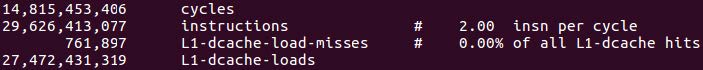
\includegraphics[width=0.9\textwidth]{content/1/chapter4/images/12.jpg}\\
图4.12 - 测试良好的使用L1缓存的程序
\end{center}

将内存大小增加到128MB意味着缓存未命中非常频繁:

%\hspace*{\fill} \\ %插入空行
\begin{center}
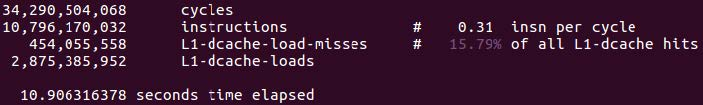
\includegraphics[width=0.9\textwidth]{content/1/chapter4/images/13.jpg}\\
图4.13 - 测试未良好的使用L1缓存的程序
\end{center}

请注意,\texttt{perf stat}收集整个程序的测量值,其中一些内存访问是缓存高效的,一些则不是。我们想知道哪里对内存访问的处理很糟糕,可以使用\texttt{perf record}和\texttt{perf report}获得详细的配置文件,如第2章所示(在那里使用了不同的计数器,但是我们选择收集计数器的过程是相同的)。当然,如果最初的配置文件没有检测到任何热代码,缓存配置文件也会显示同样的结果。代码中的许多位置,缓存未命中的比例都很大。每个位置只对总体执行时间没什么贡献,但这会累积。现在我们注意到,这些代码位置中的许多都有一个共同点:所操作的内存,例如:若它们之间有几十个不同的函数,总共占15\%的缓存未命中率,但是它们都在同一个列表上运行,那么这个列表就是有问题的数据结构,我们必须以其他方式组织我们的数据。

我们现在已经了解了如何检测和识别那些低效的内存访问模式,和会对性能产生负面影响的数据结构,以及有哪些替代方案。不幸的是,可供选择的数据结构通常没有相同的特性或性能:如果从数据结构的整个生命周期来看,必须在任意位置插入元素,则不能用\texttt{vector}替换\texttt{list}。若不是数据结构,而是算法本身调用了低效率的内存访问,则需要改变算法。

\subsubsubsection{4.5.3\hspace{0.2cm}优化内存性能的算法}

算法的内存性能会经常忽视。选择算法,通常根据其\textbf{算法性能}或执行的操作或步骤的数量来。内存优化通常需要反直觉的选择:做更多的工作,甚至不必要的工作,以提高内存性能。这里是用一些计算来换取更快的内存操作。内存操作很慢,所以要做的工作也很多。

更快地使用内存的方法是使用更少的内存,这种方法通常会需要重新计算一些本可以存储和从内存中检索的值。最坏的情况是,如果检索结果需要随机访问,读取每个值需要几纳秒(在我们这是7纳秒)。重新计算这个值所花费的时间比这要少,而将7纳秒转换为CPU可以执行的操作数是相当长的时间,那么我们最好不存储这些值。这是传统的空间与内存的权衡。

这种优化有一个有趣的变式:在给定时间内使用更少的内存,而不是简单地使用更少的内存。这里的想法是想将当前工作的数据集放入缓存中,比如L2缓存,并在移动到数据的下一部分之前对它进行尽可能多的处理。根据定义,将新数据集插入到缓存中会导致内存地址的缓存未命中。最好接受这一次缓存未命中,然后在一段时间内有效地操作数据。而非一次处理所有数据,并在每次需要此数据元素时,会有缓存未命中的风险。

这一章,将展示一种更有趣的技术,通过更多的内存访问来保存一些其他的内存访问。这里的权衡不同:希望减少缓慢的、随机的访问次数,但是我们增加了快速的、连续的访问次数。由于顺序内存流比随机访问快一个数量级,我们还有很多必须做的额外工作,以减少缓慢的内存访问。

演示需要一个更详细的示例。假设我们有一组数据记录,比如字符串,程序需要对其中一些记录进行一些更改。然后我们得到另一组的变化,以此类推。每个集合将对某些记录进行更改,而其他记录保持不变。通常,这些变化会改变记录的大小及其内容。在每个集合中更改的记录子集是完全随机和不可预测的。以下是一张演示图表:

%\hspace*{\fill} \\ %插入空行
\begin{center}
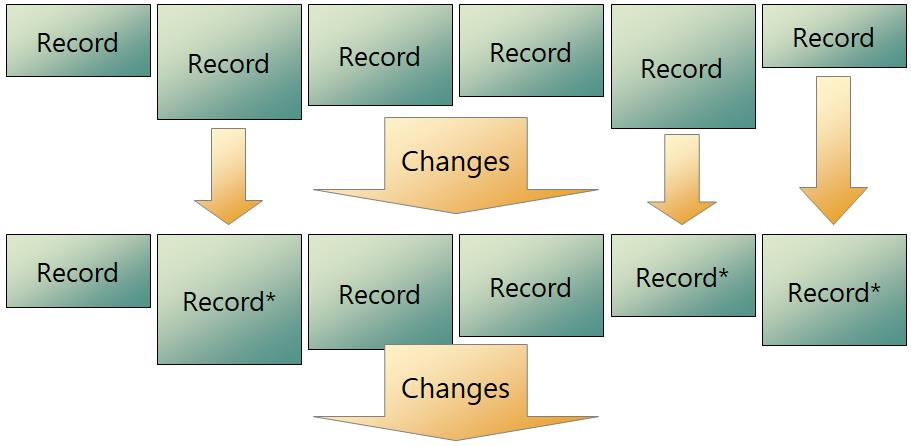
\includegraphics[width=0.9\textwidth]{content/1/chapter4/images/14.jpg}\\
图4.14 - 记录编辑问题。在每个变更集中,由*标记编辑过的记录,其余的保持不变
\end{center}

解决这个问题最简单的方法是将记录存储在它们自己的内存分配中,并将它们组织在某种数据结构中,允许新记录的替换(因为新记录的大小通常不同,需要重新分配旧记录)。数据结构可以是树(在C++中设置)或列表。为了让这个例子更加具体,我们使用字符串作为记录,还必须说明更改集的指定方式。它没有指向需要更改的特定记录,但对于任何记录,我们都可以说它是否需要更改。这种字符串更改集的最简单示例是查找和替换模式。这里,可以概述我们的实现:

\begin{lstlisting}[style=styleCXX]
std::list<std::string> data;
… initialize the records …
for (auto it = data.begin(), it0 = --data.end(), it1 = it;
true; it = it1) {
	it1 = it;
	++it1;
	const bool done = it == it0;
	if (must_change(*it)) {
		std::string new_str = change(*it);
		data.insert(it, new_str);
		data.erase(it);
	}
	if (done) break;
}
\end{lstlisting}

每个更改集中,我们都遍历整个记录集合,确定是否需要更改记录,如果需要,就这进行变更(更改集隐藏在函数\texttt{must\_change()}和\texttt{change()}中)。代码只显示一个更改集,因此我们需要运行这个循环多次。

这个算法的缺点是使用了列表,更糟的是一直在内存中移动字符串。对新字符串的访问会出现缓存未命中。如果字符串非常长,那么初始的缓存未命中就不重要了,其余的字符串都可以使用顺序访问快速的进行读取。结果与前面的块分配数组相似,而且内存性能良好。如果字符串很短,那么整个字符串很可能在一次加载操作中读取,并且每次加载都是在一个随机地址上进行。

整个算法只在随机地址处做加载和存储。我们已经知道,这是访问内存最糟糕的方法。那我们能做什么呢?不能将字符串存储在巨大的数组中:如果数组中间的字符串需要增长,那么内存从哪里来?该字符串后面的一个字符串,所以这里已经没有增长的空间了。

想出一个替代方案,不过需要范式转换。按字面意思执行所需操作的算法也对内存组织施加了限制:更改记录需要将它们移动到内存中,而且我们希望能够在不影响其他东西的情况下更改记录,所以我们就不能避免内存中记录的随机分布。我们必须从侧面来看待这个问题,从限制开始。按顺序访问所有的记录,在这个约束条件下我们能做什么?我们可以很快地读取所有记录。可以决定记录是否必须更改,这一步和之前一样。如果记录必须增加,该怎么办?必须把它移到别的地方去,这些记录要按照先后顺序分配。然后,前一个记录和下一个记录也必须移动,因此它们在新记录之前和之后都保持存储状态。这是替代算法的关键:所有记录都随着每个变更集移动,无论它们是否更改。我们可以将所有记录存储在一个巨大的连续缓冲区中(假设我们知道总记录大小的上限):

%\hspace*{\fill} \\ %插入空行
\begin{center}
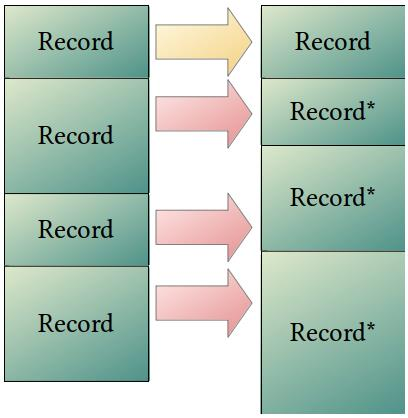
\includegraphics[width=0.25\textwidth]{content/1/chapter4/images/15.jpg}\\
图4.15 - 按顺序处理所有记录
\end{center}

算法要求在复制过程中分配大小相等的第二个缓冲区,因此内存消耗峰值是数据大小的两倍:

\begin{lstlisting}[style=styleCXX]
char* buffer = get_huge_buffer();
… initialize N records …
char* new_buffer = get_huge_buffer();
const char* s = buffer;
char* s1 = new_buffer;
for (size_t i = 0; i < N; ++i) {
	if (must_change(s)) {
		s1 = change(s, s1);
	} else {
		const size_t ls = strlen(s) + 1;
		memcpy(s1, s, ls);
		s1 += ls;
	}
	s += ls;
}
release(buffer);
buffer = new_buffer;
\end{lstlisting}

在每个更改集中,我们将每个字符串(记录)从旧缓冲区复制到新缓冲区。如果需要更改记录,则将新版本写入新的缓冲区;否则,原作将复制。对每个新的更改集,创建一个新的缓冲区,并在操作结束时释放旧的缓冲区(实际的实现需要避免重复调用分配和释放内存,并简单地交换两个缓冲区)。

这种实现的明显缺点是使用巨大的缓冲区:我们必须确定缓冲区的大小,以便为可能遇到的最大记录分配足够的内存。峰值内存的大小也令人担忧。我们可以通过将这种方法与前面看到的可增长数组数据结构相结合来解决这个问题。可以将记录存储在一系列固定大小的块中,而不是分配一个连续的缓冲区中:

%\hspace*{\fill} \\ %插入空行
\begin{center}
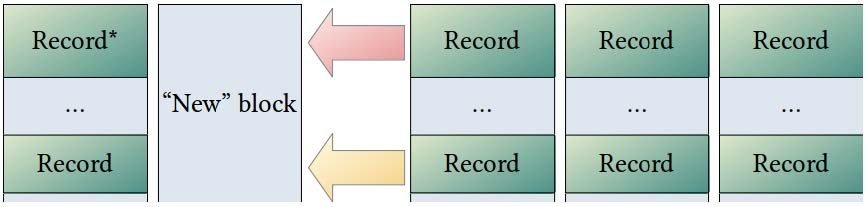
\includegraphics[width=0.9\textwidth]{content/1/chapter4/images/16.jpg}\\
图4.16 - 使用块缓冲区进行编辑
\end{center}

为了简化图表,我们绘制了相同大小的所有记录,但是这个限制是不必要的:记录可以跨越多个块(我们将这些块视为一个连续的字节序列,仅此而已)。当编辑时,我们需要为已编辑的记录分配一个新块。编辑完成后,可以释放包含旧记录的块(或多个块),从而不必等待读取整个缓冲区。可以做得更好:我们可以将最近释放的块放到空块列表中,而不是返回操作系统。即将编辑下一个记录,我们将需要一个空的新块作为结果。只是碰巧有一个:这是块用来包含我们编辑的最后一个记录。它位于最近发布的块列表的头部,最重要的是,这个块是我们访问的最后一块内存,所以它可能仍然在缓存中!

乍一看,这个算法似乎非常糟糕:每次都要复制所有的记录。让我们更仔细地分析这两种算法。首先,读取的数量相同:两种算法都必须读取每个字符串,以确定是否更改。第二种算法在性能上已经领先:在一次连续扫描中读取所有数据,而第一种算法则在内存中跳跃。如果编辑该字符串,那么两个算法都必须向新的内存区域写入一个新的字符串。由于顺序内存访问模式(同样,不需要为每个字符串执行内存分配),第二种算法提前出现了。当字符串未编辑时,就需要进行权衡。第一个算法什么都不做,第二个做了一个拷贝。

通过这种分析,我们可以为每个算法定义好的和坏的情况。如果字符串很短,并且在每个更改集中更改了大部分字符串,则顺序访问算法胜出。如果字符串很长或者很少改变字符串,随机访问算法就会获胜。然而,确定什么是长、多少是大比例的唯一方法就是测试。

这里,不一定意味着必须编写完整程序的两个版本进行测试。通常,可以对简化数据进行操作的小型模拟程序中模拟特定的行为。我们只需要知道记录的大致大小,有多少条更改记录,并且需要对单个记录进行更改的代码,这样就可以测量内存访问对性能的影响(如果每次更改影响都非常大,那么读取或写入记录所花费的时间就无关紧要了)。可以对这样的模拟或原型实现进行近似测量,并做出正确的设计决策。

在现实中,顺序字符串复制算法值得一试么?我们已经完成了使用正则表达式模式编辑中等长度字符串(128字节)的测试。所有字符串的99\%都在每个更改集中进行编辑,顺序算法的速度大约是随机算法的4倍(结果在某种程度上是特定于机器的,因此必须在与预期使用的硬件相似的硬件上进行测量)。编辑了50\%的记录时,顺序访问仍然更快,但是只有12\%的性能提升(这可能是在不同的CPU模型和内存类型的变化范围内,所以我们称之为平局)。更令人惊讶的结果是,如果只更改了1\%的记录,那么这两种算法的速度几乎是成正比的:不进行随机读取所节省的时间将用来弥补完全不必要的复制。

较长的字符串,随机访问算法轻松获胜,如果改变很少的字符串,而且对于非常长的字符串,即使所有的字符串都改变,也是平局:两种算法都依次读取和写入所有字符串(对长字符串开始的随机访问增加的时间可以忽略)。

现在我们已经掌握了应用程序所需的所有算法。性能设计通常是这样的:确定性能问题的根源,并想出消除问题的方法,但代价是要做其他更多事情,然后必须创造一个测试,让我们能够衡量这个技巧是否真的有效。

本章的最后,将向您展示一个完全不同的“使用方式”,由缓存和其他硬件提供的性能改进。




























